\documentclass{ximera}

\title{Tutorial}

\begin{document}
\begin{abstract}
  This course is built on this platform, Ximera.
\end{abstract}

Mathematics cannot be learned passively: it must be actively
\href{http://en.wikipedia.org/wiki/Constructivism_(philosophy_of_education)}{constructed}
by the mind of the person learning it.  With this in mind, this course
is built around solving problems!

Here is an example problem.  Play around with it, get it wrong, try
the hints out.  Don't be afraid to fail: getting an answer wrong never
hurts you.

\begin{problem}
  \begin{solution}
    \begin{hint}
      $3 \times 2$ is the number of objects in $3$ groups of $2$ objects
    \end{hint}
    \begin{hint}
      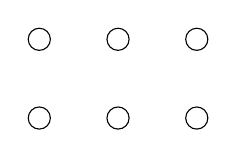
\begin{tikzpicture}
        \draw (0,0) circle (4pt);
        \draw (1,0) circle (4pt);
        \draw (2,0) circle (4pt);
        \draw (0,1) circle (4pt);
        \draw (1,1) circle (4pt);
        \draw (2,1) circle (4pt);
      \end{tikzpicture}
    \end{hint}
    \begin{hint}
      $3\times 2=6$
    \end{hint}
    $3\times 2 = $ \answer{6}
  \end{solution}
\end{problem}

Even if you get an answer right you should \textit{always} try the
hints out afterwards.  They might explain the concept from a new point
of view, or challenge you to think in a different way than you solved
the problem.
\\
\\
We support a few different answer types: as you have seen above,
numerical answers are one type.  Here are some example problems from
the different answer types we support:
\\
\\

\begin{problem}
  \textbf{An expression answer type}
  \begin{solution}
    \begin{hint}
      Great!  You looked at this hint.  That is totally what you were supposed to do.
    \end{hint}
    \begin{hint}
      Sometimes hints have problems in them.  Usually these problems would be a simpler version of the question you are trying to answer,
      or a crucial part of the solution.  In this case, it is just a demo of problems within hints:
      \begin{question}
        The last sultan of the Ottoman Empire was:
        \begin{solution}
          \begin{hint}
            Check Wikipedia!
          \end{hint}
          \begin{hint}
            The correct answer is Abdülmecid II.
          \end{hint}
          \begin{multiple-choice}
            \choice[correct]{Abdülmecid II}
            \choice{Abdülhamid II}
            \choice{Suleiman II}
          \end{multiple-choice}
        \end{solution}
      \end{question}
    \end{hint}
    Try writing the expression $x^2+y$ = \answer{x^2+y}.  Remember to try failing as well, to see what happens.
  \end{solution}
\end{problem}

\begin{problem}
  \textbf{A matrix answer type}
  \begin{solution}
    \begin{hint}
      Just making sure you are still clicking on these!
    \end{hint}
    Try inputing the matrix $\begin{bmatrix}  0&1\\2&3\\0&0\end{bmatrix}$ here
    \begin{matrix-answer}[name=M]
      correctMatrix = [['0','1'],['2','3'],['0','0']]
    \end{matrix-answer}
  \end{solution}
\end{problem}

A free response answer type:

Tell us who you are and why you are taking this course!
\begin{free-response}
  We are Steven Gubkin and Jim Fowler, and we are writing this course because we loving sharing mathematics with others!
\end{free-response}

You may have noticed that as you complete activities you get more ``Xudos'' (at the top of the page).  These are points, and people love points.
There is another kind of points called ``Xarma'' which you get for engaging with the community by making forum posts, reviewing someone elses work, or 
helping to make the course better by contributing to our \href{https://github.com/kisonecat/m2o2c2}{github page}.

As you complete activities the green ``completion bar'' also moves at
the top of the page.  This lets you know how close you are to being
done.

You can comment on this page at the very bottom: try it out!

You advance through pages either by completing them and clicking the
``next activity'' button, or by navigating on the little side panel to
the right.  Every time you complete an activity ou get a green check
mark on the side panel, to let you know you have already done it.
 
Only one more question left:
\begin{question}
  \begin{solution}
  
    Are you ready to start learning some Calculus!?!
    \begin{hint}
        We promise the real course will not be this corny.
      \end{hint}
    \begin{multiple-choice}
      \choice[correct]{Yes I am!}
    \end{multiple-choice}
  \end{solution}
\end{question}

Oh ya, we also embed videos
\youtube{http://www.youtube.com/watch?v=K7yICPCEOFw}

\end{document}